\chapter{Algnment Examples}\label{appendix-a}

I would like to shortly compare the  alignments computed by eflomal and SimAlign with my annotations from the gold standard, especially regarding some of the examples I mentioned in Section~\ref{sec:gold-standard-examples} for handling ambiguous cases.

I will consider the following cases: double negation, German preterit vs.~Romansh perfect and composite words.



Below are some examples for word alignment of the different systems. 
Green squares are the gold standard, circels are SimAlign and boxes are eflomal.

\begin{figure}[ht]
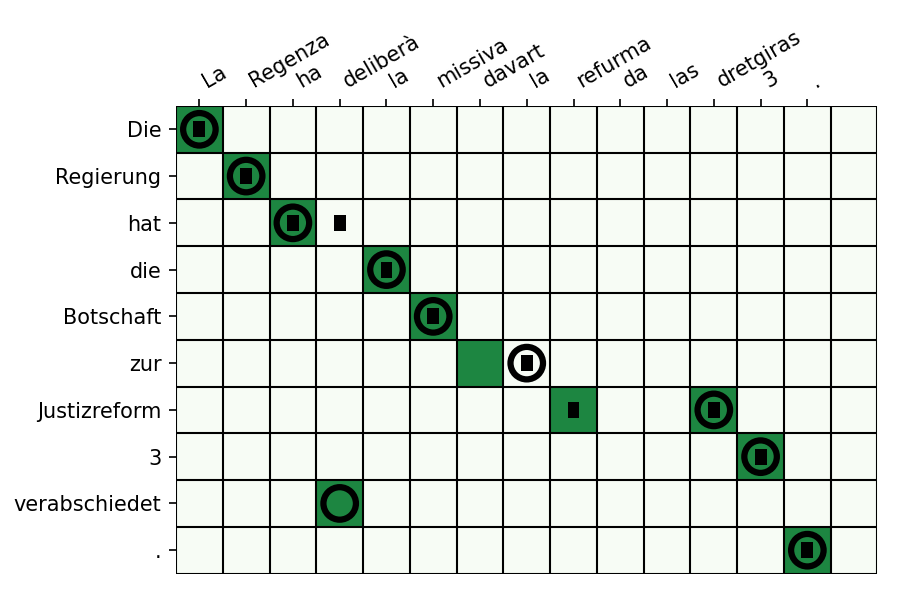
\includegraphics{graphics/alignments/example1.png}
\caption{Word alignment example 1}
\end{figure}

\begin{figure}[ht]
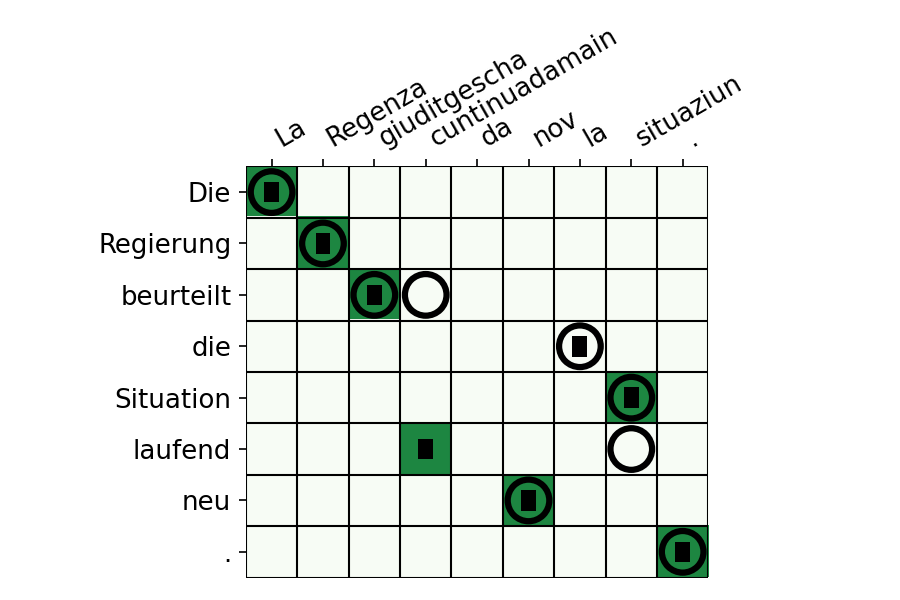
\includegraphics{graphics/alignments/example2.png}
\caption{Word alignment example 2}
\end{figure}

\begin{figure}[ht]
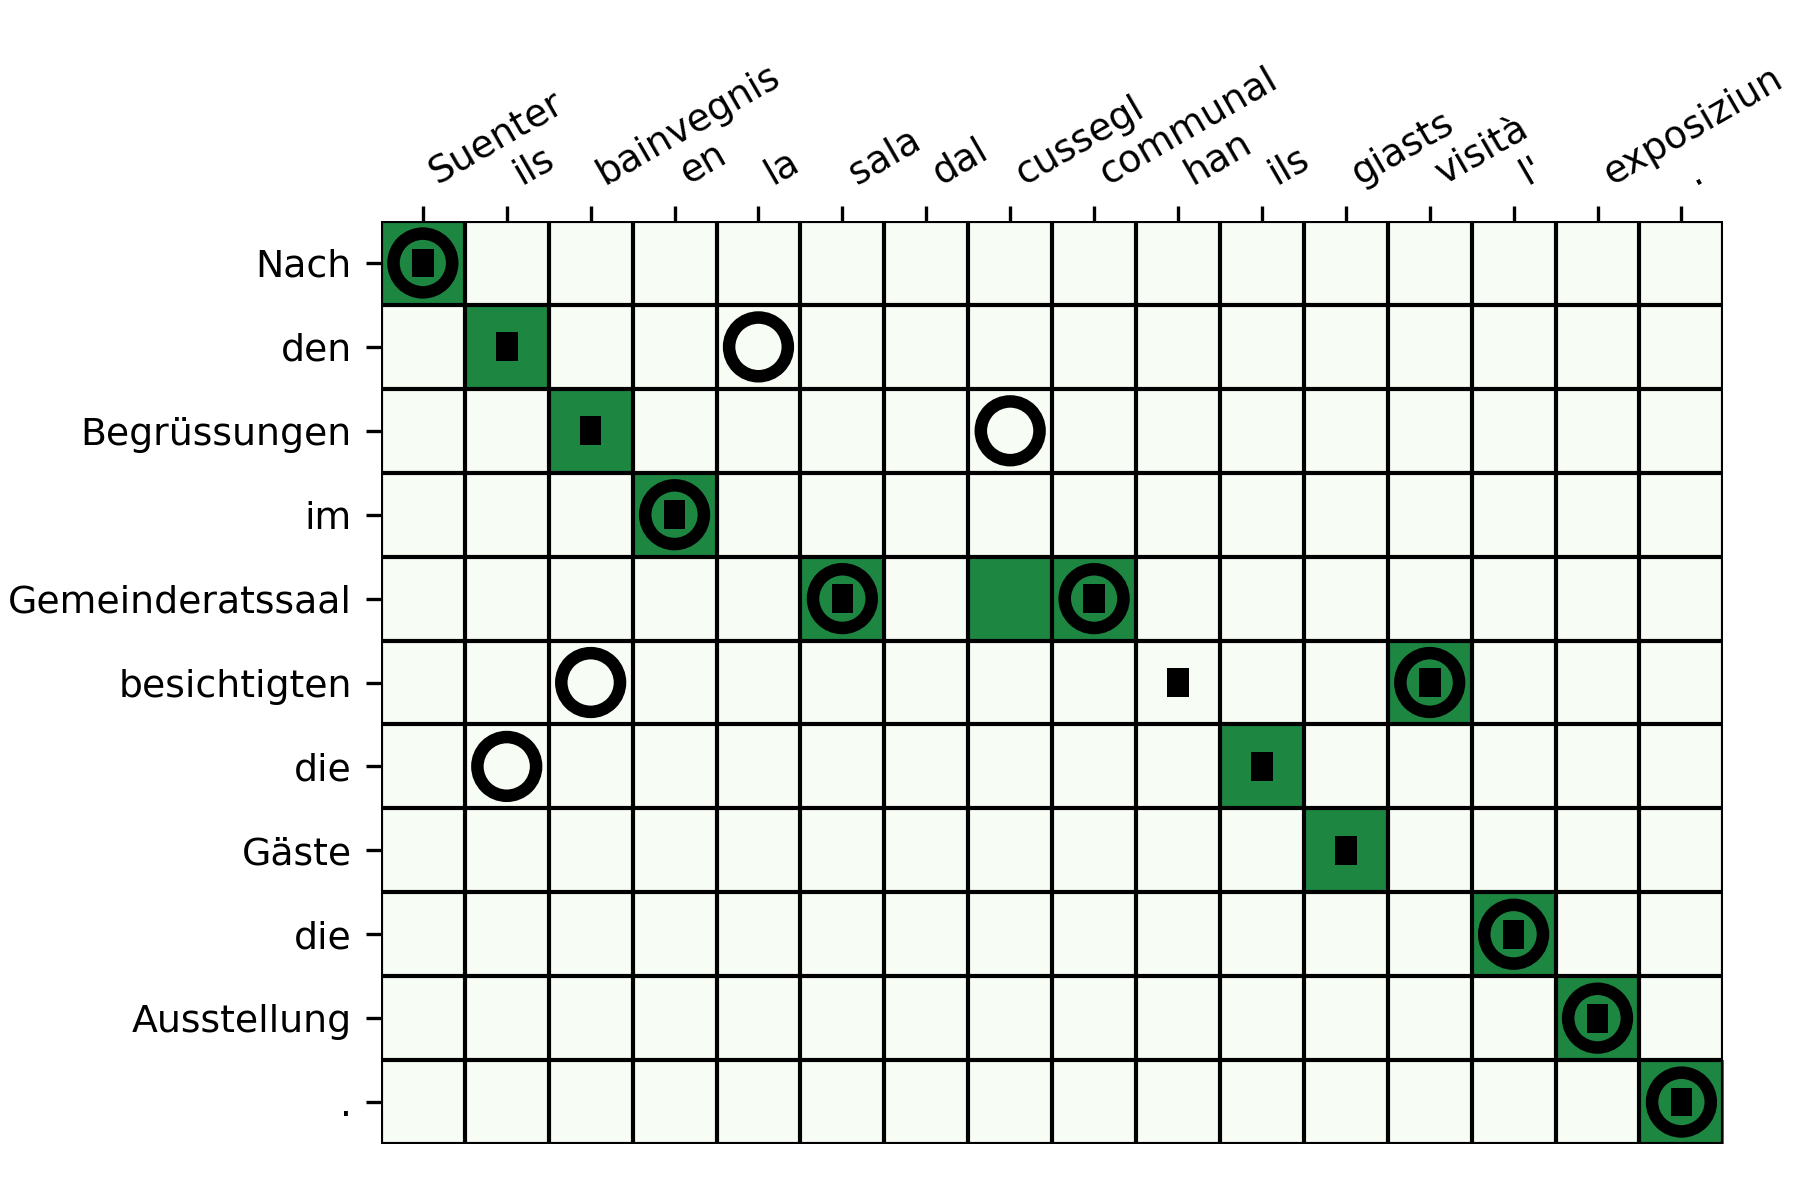
\includegraphics{graphics/alignments/example3.png}
\caption{Word alignment example 3}
\end{figure}

\begin{figure}[ht]
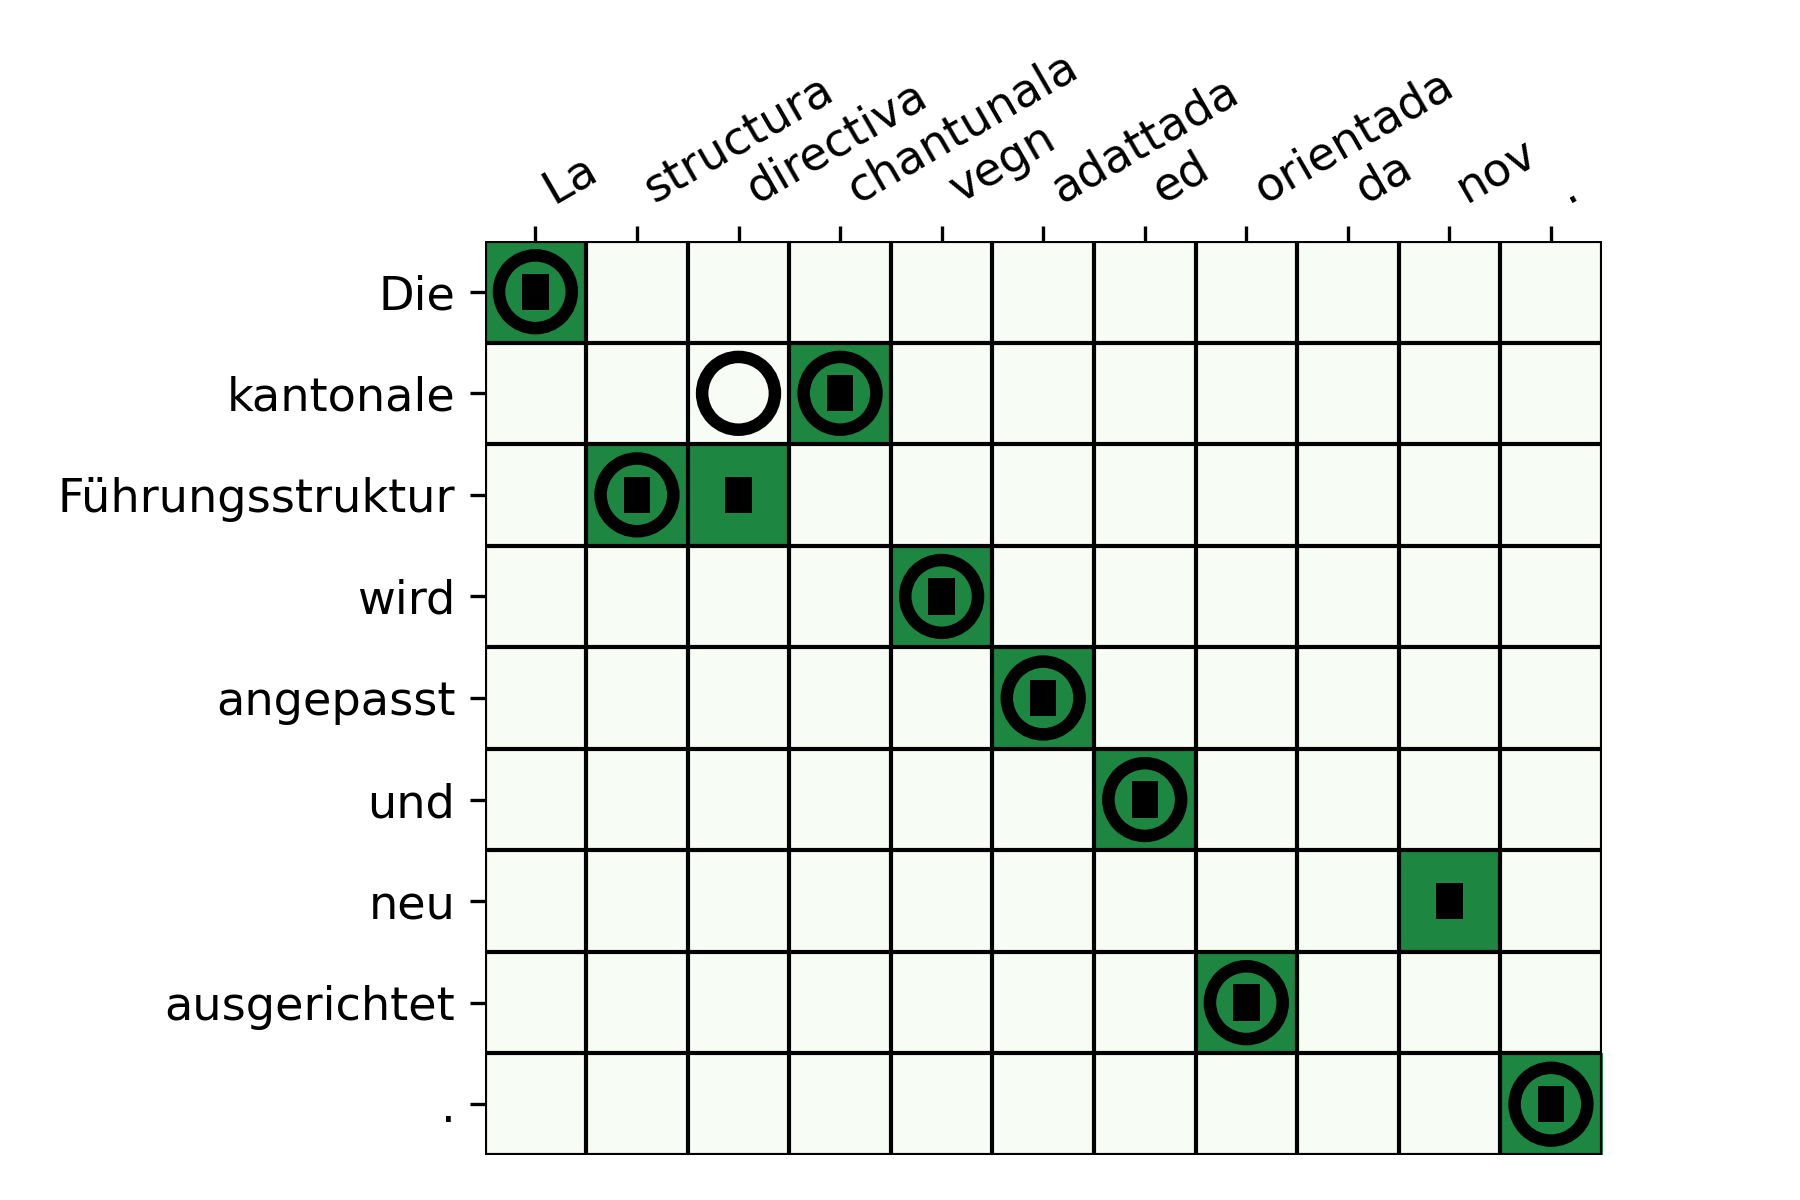
\includegraphics{graphics/alignments/example4.png}
\caption{Word alignment example 4}
\end{figure}

\begin{figure}[ht]
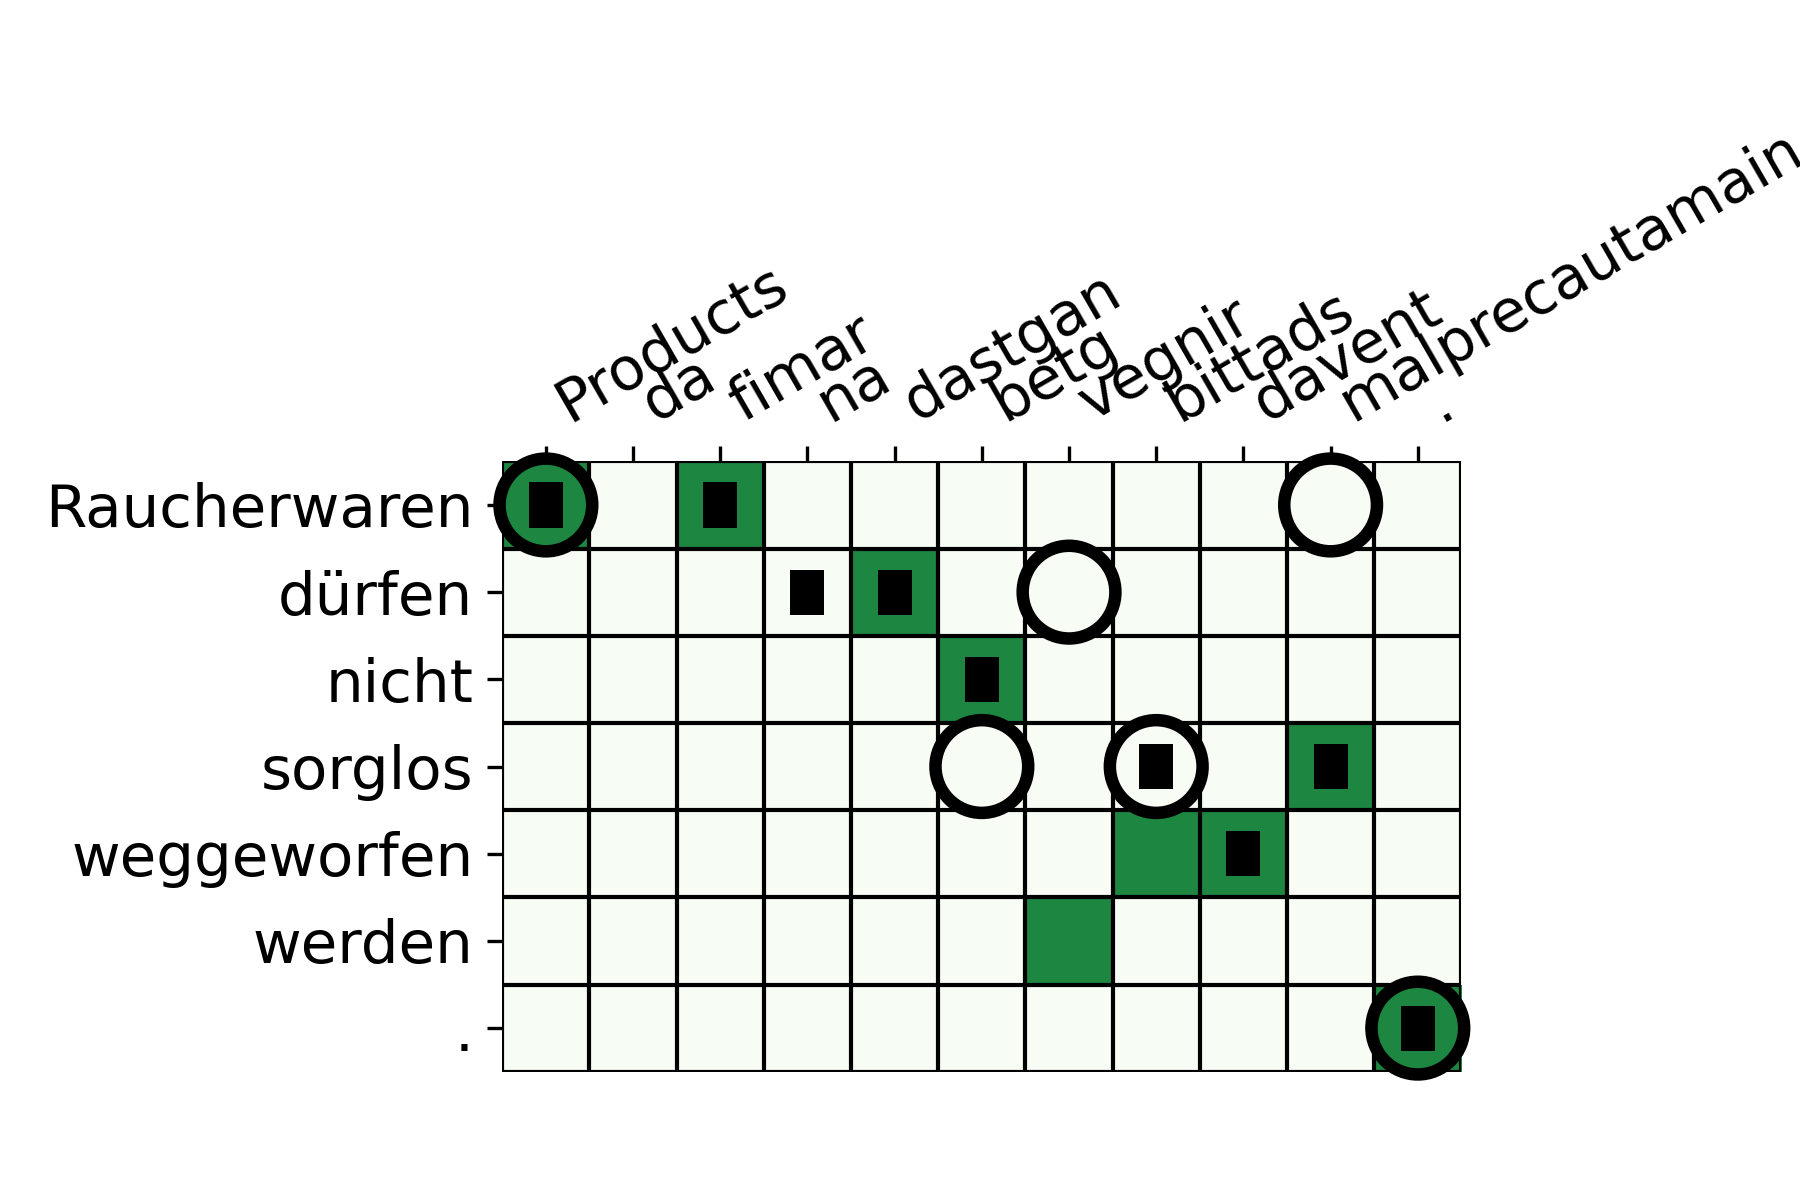
\includegraphics{graphics/alignments/example5.png}
\caption{Word alignment example 5}
\end{figure}